%
%  --- USU thesis and dissertation template ---
%

\documentclass[ee,dissertation,x11names,table]{nyuthesis}
%{{{ Packages
\usepackage{amssymb}           % add ams symbols stuff
\usepackage{graphicx}          % add graphics
%\usepackage{subfigure}
\usepackage{url}

\usepackage{subcaption}
%\usepackage{flafter}           % Cause floats to appear after
                               % environment.
%\usepackage{siunitx}           % Provides standard formatting of SI units.

% Include TikZ and PGF packages for high-quality graphics, schematics
% and plots. This is optional; at the current time, when run with
% latex to create a .dvi file, the xdvi viewer will produce incorrect
% formatting for the TikZ figures.  If the .dvi file is converted to
% pdf using "dvipdf" the resulting pdf file is correct.  If this
% example is used with  pdflatex, the resulting TikZ figures in the
% output look fine.
\usepackage{tikz}       		% The base tikz+pgf package
\usetikzlibrary{arrows,shapes}	% Optional tikz extensions
\usepackage[american]{circuitikz}	% TikZ-based package for schematic drawings
\usepackage{pgfplots}			% Tikz-based package for making plots 
\pgfplotsset{compat=1.6}        % This *might* be necessary for your
                                % version of pgfplots.

\usepackage{hyperref} % Creates hyperlinks within document
\hypersetup{colorlinks=true, linkcolor=blue,
  citecolor=blue,urlcolor=blue} % Use when compiling the digital copy
% \hypersetup{colorlinks=true, linkcolor=black,
% citecolor=black,urlcolor=black} % Use when compiling the printed copy

% The following allows for hyperlinked DOIs to be inserted in the
% manuscript by using \doi{}.
\usepackage{doi}

% Set spacing around figures and tables to triple space
\setlength{\intextsep}{2em} % Vertical space above & below [h] floats
\setlength{\textfloatsep}{2em} % Vertical space below (above) [t] ([b]) floats

% The following is added if you are using the multiple-paper format to
% add references after each chapter:
%\usepackage[sectionbib]{chapterbib}

%}}}

% Author and Title Information
\author{Parvez A. Kose}
\title{Explainable Deep Learning and Visual Interpretability}

% The Committee
\majorprof{Elizabeth P. Henaff, Ph.D.}
\departmentname{Technology, Culture and Society}
\firstreader{Gene Kogan, B.Sc}
\secondreader{Tega Brain, M.A}
\thirdreader{Jack Craig Toolin}
\fourthreader{}

% Graduate Dean
\graddean{}
\deantitle{Department Chair}

% Degree Information
%\degree{Master of Science}
\doctype{thesis}
\degree{Masters of Science}
\degreein{INTEGRATED DIGITAL MEDIA}
\month{May}
\gradyear{2019}

\begin{document}
    %{{{ Frontmatter
    \preliminaries   % set frontmatter style
    
    \maketitle
    %\makecopyright        % optional
    
    %
%  Time-stamp: "[abstract.tex] last modified by Scott Budge (scott) on 2017-01-10 (Tuesday, 10 January 2017) at 16:54:14 on goga.ece.usu.edu"
%
%  Info: $Id: abstract.tex 998 2017-03-21 16:44:33Z scott $   USU
%  Revision: $Rev: 998 $
% $LastChangedDate: 2017-03-21 10:44:33 -0600 (Tue, 21 Mar 2017) $
% $LastChangedBy: scott $
%

\begin{abstract}
% A space is needed before the text starts so that the first paragraph
% is indented properly.

Deep learning a branch of machine learning has seen a revolutionary improvement in many areas such as voice recognition, computer vision and natural language processing. It is being used to guide all sorts of crucial decisions in medicine, finance, manufacturing and beyond, including deciding who gains access to healthcare, who gets approved for a loan and who gets hired for a job. However, do we understand how these systems work? Are they trustworthy? Can we detect bias in their models? The lack of explanation regarding the model decisions and absence of control over their internal processes act as a critical impediment. I discuss the societal implications of black box models and the need for interpretable and explainable systems. This work propose visualization techniques that justify the prediction of a visual classificators by providing visual evidence for their decision, namely: (i) Sensitivity analysis to  show which part of the  input image  is  most  relevant  to  the  classification decision, and (ii) Activation graph visualizing intermediate outputs to get a better insight on what the network has learned. Finally, I discuss the exigency to address the issue of transparency, accountability and fairness in the AI system, and ensure that bias in the data doesn't get embedded in the systems we create.

\end{abstract}


% Local Variables:
% TeX-master: "newhead"
% End:

    %
%  Time-stamp: "[publicabstract.tex] last modified by Scott Budge (scott) on 2011-08-09 (Tuesday, 9 August 2011) at 09:17:43 on goga"
%
%  Info: $Id$   USU
%  Revision: $Rev$
% $LastChangedDate$
% $LastChangedBy$
%

\begin{publicabstract}
% A space is needed before the text starts so that the first paragraph
% is indented properly.

Deep learning, a branch of machine learning has led to breakthrough and innovation in many areas such as computer vision, voice recognition and natural language processing. It is being used to guide all sorts of business decisions, both routine and high stakes because they promise to improve the quality and consistency of decision making. These techniques have been embraced in the regulated domain, where decisions like who gains access to healthcare, approved for a loan and who gains access to critical opportunities depends on the output of the deep learning models. There is a growing perception that these learning algorithms from historical data can end up encoding human biases and prejudice they promised to alleviate. With the increasing complexity of deep learning models and their influence on the public domain, the critical need for understanding their inner-workings has increased. I discuss the societal implications of the black box models and the corresponding need to address the issue of transparency and fairness. I provide an overview of the deep learning visualization research, and the recent efforts to make deep learning models interpretable and explainable. This works uses explainable system approach together with image localization and visualization techniques to interpret the decision of a visual classification task that justifies the model decision using visual evidence, using the following methods: (i) Sensitivity analysis to show which part of the image attributed to the classification decision, and (ii) Activation graph visualizing intermediate outputs of the network to understand what the network has learned. Finally, I discuss the exigence to address the issue of transparency, accountability and fairness in the AI system, and ensure that bias in the data doesn't get embedded in the systems we create.

%This work is a contribution towards promoting transparency and fairness and building a fair, safe and equitable AI system.

\end{publicabstract}


% Local Variables:
% TeX-master: "newhead"
% End:

    %%
% This is an example of an dedication page.  This is optional,
% and can contain anything you want to say.
%
%  Time-stamp: "[dedication.tex] last modified by Scott Budge (scott) on 2011-08-08 (Monday, 8 August 2011) at 15:46:26 on goga"
%
%  Info: $Id$   USU
%  Revision: $Rev$
% $LastChangedDate$
% $LastChangedBy$
%

\begin{dedication}
\begin{center} 
%To all the little people....
\end{center}
% 
% If you intend to have a dedication longer than one line, do not put
% it in a centering environment.  It will look better.
\end{dedication}
  % optional 
    %
% This is an example of an acknowledgements page.  This is optional,
% and can contain anything you want to say.
%
%
%  Time-stamp: "[acknowl.tex] last modified by Scott Budge (scott) on 2011-08-08 (Monday, 8 August 2011) at 15:45:15 on goga"
%
%  Info: $Id$   USU
%  Revision: $Rev$
% $LastChangedDate$
% $LastChangedBy$
%

\begin{acknowledgments} 

This work would not have been realized without the help and support of the following people who graciously contributed to the work presented in this thesis.

Firstly, I would like to express my sincere gratitude to my advisor Prof. Gene Kogan for the continuous support of my thesis study and research, for his patience, encouragement, immense knowledge and expertise. I could not have imagined having a better mentor and advisor for my thesis study.

Besides my advisor, I would like to express my immense gratitude to my thesis professor Dr. Elizabeth P. Henaff. Her counsel and guidance helped me all through the research process and writing of this thesis. Without her continued guidance and stewardship, it would not have been possible to conduct this research.

I am truly grateful to Prof. Daniel Shiffman who took time to discuss my work and share his constructive feedback which inspired me to widen my research from various perspectives. I also would like to extend my special thanks to Prof. Tega Brain for her insightful feedback and helping perfect this thesis paper.

I also would like to thank my pre-thesis instructor, Prof. Dana Karwas and Prof. Benedetta Piantella for helping shape the research and providing useful insight when the project was in its nascent stage.

I also would like to thank the rest of my thesis committee, mentors and advisors: Prof. Jack Toolin, Prof. Mark Skwarek and Prof. Luke DuBois for their insightful remarks and encouragement.

Finally, I thank my fellow peer in for the stimulating discussions and user testing for the prototype, and all the collaboration and learning. Also, I would like to thank my friends in the following institution: NYU Tandon School of Engineering and NYU Center For Data Science. %In particular, I am grateful to Prof. Iddo Drori for enlightening me the first glance of the research.

%Finally, I would like to thank my family for supporting me generously throughout this thesis coursework.
\vspace*{-1em}
\begin{flushright} 
Parvez A. Kose
\end{flushright}
\end{acknowledgments}


     % optional
    
    \tableofcontents 
    \listoftables 
    \listoffigures
    
%    %
%  Time-stamp: "[notation.tex] last modified by Scott Budge (scott) on 2011-08-08 (Monday, 8 August 2011) at 15:48:03 on goga"
%
%
% This is an example of a notations page.  
% The publication guide does not specify a format.
% The example here is in tabular format.
%
% Please note that the symbols in this example are defined
% in a separate include file.
%  Info: $Id$   USU
%  Revision: $Rev$
% $LastChangedDate$
% $LastChangedBy$
%

\begin{notation}

\setlength{\tabcolsep}{3mm}
{\begin {tabular}{ll}
\multicolumn{2}{l}{\textbf{Events}}\\
$\Sigma$ & set of all events (universal alphabet)\\
$\tick$   & successful termination signal\\
$\tau$ & invisible (internal) event\\
$a.b.c$    & compound event\\
$c ? x$   &input on channel $c$\\
$c ! x$   &output on channel $c$\\
$\lchan c \rchan$   &set of all events associated with channel $c$\\
\multicolumn{2}{l}{\textbf{Traces}}\\
$\nil$ &empty sequence\\
$\lseq a_1, \ldots , a_n \rseq$ & sequence $a_1, \ldots , a_n$, in that order\\
$s_1 \cat s_2$ &$s_1$ concatenated with $s_2$, e.g. $\lseq a \rseq \cat \lseq b \rseq = \lseq a, b \rseq$\\
$s_1 \leq s_2$ &$s_1$ is a prefix of $s_2$, e.g.  $\lseq a \rseq \leq \lseq a, b \rseq$ \\
$s \hide X$ &hiding - all members of $X$ removed from $s$\\
$s \restrict X$ &restriction - hide all but members of $X$\\
$s \crestrict c$ &sequence of values in $s$ communicated over channel $c$\\
$s \seqcount a$ &number of $a$ events in $s$\\
\multicolumn{2}{l}{\textbf{Processes}}\\
$a \then P$ &prefixing\\
$P \interleave Q$ &interleaved parallel\\
$P \parallel[A][B] Q$ &alphabetized parallel\\
$P \parallel[X] Q$ &interface parallel\\
$P \extchoice Q$ &external choice\\
$P \intchoice Q$ &nondeterministic choice\\
$P \comp Q$ &sequential composition\\
$P \hide X$ &hiding\\
\end {tabular}}

% The table as defined above will fill one page. If you need more room to list
% notation you will need to create a second table, and place it below this 
% comment. This new table will appear one a new page.

\end{notation}

  % optional
    %
% This is an example of an acronyms page.  
% Acronyms are laid out in tabular format.
%
%  Time-stamp: "[acronyms.tex] last modified by Scott Budge (scott) on 2011-08-08 (Monday, 8 August 2011) at 15:45:41 on goga"
%
%  Info: $Id$   USU
%  Revision: $Rev$
% $LastChangedDate$
% $LastChangedBy$
%

\begin{acronyms}

\renewcommand{\arraystretch}{1.5}
\setlength{\tabcolsep}{3mm}
{\begin {tabular}{ll}

AI  &    Artificial Intelligence    \\
ML  &   Machine Learning    \\
ANN &   Artificial Neural Network   \\
DNN &   Deep Neural Network \\
CNN &   Convolutional Neural Network    \\
VGG16   &   Vector Graphic Group 16 \\
XAI &   Explainable Artificial Intelligence \\
GDPR    &   General Data Protection Regulation  \\
DARPA   &   Defense Advanced Research Projects Agency   \\
GPU &   Graphic Processing Unit
TPU &   Tensor Processing Unit

\end {tabular}}

\end{acronyms}
  % optional  
    %}}}
    %{{{ The main body of the thesis
    \body  % set main body style
    % Chapters
    %
%  This is an example of how a LaTeX thesis should be formatted.  This
%  document contains chapter 1 of the thesis.
%
\chapter{INTRODUCTION}
%%%%%%%% This line gets rid of page number on first page of text
\thispagestyle{empty}
%%%%%%%%%%%%%
%It is responsible for spearheading the latest advancement in artificial intelligence research.% 

Deep learning has led to an unprecedented breakthrough in many areas such as computer vision, voice recognition, and autonomous driving.  It has proved very powerful at solving large-scale real-world problems in recent years and adopted by many large-scale information processing applications like image recognition, speech recognition and language translation.  These same techniques will be able to diagnose deadly diseases,  make trading decisions, and do countless other things that will potentially transform many industries. 

While a deep neural network learns efficient and powerful representations, they are often considered as black box methods that perform assigned tasks for the users.  Understanding these models remains a challenge due to its inherently opaque nature and unclear working mechanism.  Without a definite understanding of how and why a model works it is difficult for a user to determine when a model works correctly, when it fails and how it might be improved. As a result, users treat the neural network as a black box and cannot explain how mapping from input to output data was done nor how performance might be improved. This lack of transparency acts as a significant drawback to their application, in practice.

Furthermore, automated decisions made by such models has far-reaching societal implications: widening inequality among class and race and underpinning bias and racial discrimination in automated decision-making system. As a result, transparency and fairness problem has been gaining more attention lately and efforts are being made to make deep learning models more interpretable and controllable by humans,  including building models that can explain their decisions, establish trust and transparency in how they behave in the real-world, detect model bias and for scientific curiosity.

Deep learning models are hard to interpret than most machine learning models as they learn representations that are complicated to extract and present in a human-readable form.  While it is plausible for certain types of models, it is indeed not entirely true for an image recognition model like a convolutional neural network (CNN).  We use a visualization technique to understand neural net inference on a given image.  The representations learned by deep neural net like CNN are highly responsive to visualization, in large part because they are representations of visual concepts.

We build a visual exploration tool that explains the rationale for a classification decision to an end user. The tool jointly predicts a class label,  and shows why the predicted label is appropriate for a given image using visual evidence. Our visualization method covers the following three components:

\begin{itemize}
\begin{enumerate}
\iffalse
\item  \textbf{Visualizing intermediate outputs}: It helps a user understands how successive layers transform their input, and to get an insight into the individual network filters. 
\fi

\item \textbf{Visualizing network filters}. It is useful to understand clearly what visual pattern or concept each filter in a network is receptive to. 

\item \textbf{Visualizing heatmaps} of class activation in an image. This step is useful to understand which part of an input image attributed most to the classification decision by localizing the object in the image.
\end{enumerate}
\end{itemize}

The following section presents chapter 1 that provides historical context and background of deep learning and cursory glance on the origin of neural networks.  Section 2.4 presents an overview of the common architectures.  Section 2.4 discusses the problem of the black box models.  Section 2.5 presents the central claim in a broader context of societal impacts.  Section 2.7 highlights the importance of explainable and interpretable systems.  Chapter 3 presents the methodologies used in the research process, including research hypothesis, experimental setup and the technical design of the prototype.

\footnote{The acronym VQ is used as an abbreviation for both vector quantization and vector
  quantizer.}
  
% TODO: For PATTERNS: Maximally Activating Patches%

%In order to build trust and transparency in these systems, we need better tools and techniques to understand and interpret deep neural networks; techniques to see through the black box models%

%Several methods have been developed to understand what a DNN has learned [17], [18]. In deep learning visualization research, a large body of work is dedicated to visualizing particular neurons or neuron layers [1], [19]–[20][21][22][23][24] and learned parameters, We focus here on methods that visualize the impact of particular regions of a given and fixed single image for a prediction of this image%

%why people want to visualize deep learning is to understand how deep learning models make decisions and what representations they have learned, so we can place trust in a model [60]. This notion of general model understanding has been called the interpretability or explainability when referring to machine learning models%

% s. In order to build trust in intelligent systems and move towards their meaningful integration into our everyday lives, it is clear that we must make ‘transparent’ models that explain why they predict what they predict. 
%

%interpretation to qualitatively evaluate and support the model’s predictions and create new interpretable methods for deep learning models.%

%with a focus on interpretability. These works use visualization to explain, explore, and debug models in%

%Deep learning models are hard to interpret as they learn representations that are difficult to extract and present in a human-readable form. While this is partially true for certain types of models, it is indeed not true for convolutional neural network (CNN). We use visualization techniques to interpret an image classification task. The representations learned by convnet are highly amenable to visualization, in large part because they are representations of visual concepts.%

% WHILE MOST OTHER WORK look for training phase ans saliency maps%

\iffalse
It also limits the usage and acceptance of artificial neural networks in applications involving high stake decision making, especially in regulated industries where it is demanded to use techniques that can be understood and validated.
\fi


%What are the intermediate features looking for?%
    %%%%%%%% This line gets rid of the page number on the first page of text

\begin{table}
\begin{adjustwidth}{-1cm}{}
\renewcommand\arraystretch{2.5}\arrayrulecolor{LightSteelBlue3}
\captionsetup{singlelinecheck=false, font=blue, labelfont=sc, labelsep=quad}
\caption{Timeline}\vskip 0ex

\begin{tabular}{@{\,}r <{\hskip 0ex} !{\foo} >{\raggedright\arraybackslash}p{14cm}}
\toprule
\addlinespace[0ex]

1943 & McCulloch and Pitts proposed the McCulloch-Pitts neuron model.    \\

1949 & Hebb postulated the first rule for self-organized learning. \\

1956 & The Dartmouth Artificial Intelligence Summer Research Project, a seminal AI event that motivated a generation of scientists to explore potentials of computing to match the human capabilities. \\

1962 & Frank Rosenblatt introduced the simple single layer neural network called Perceptron - the precursor of today’s learning algorithms for deep neural networks. \\

1962 & David Hubel and Torsten Wiesel published their work on Receptive Fields and Functional Architecture in the Cat’s Visual Cortex," which revealed the pattern of organization of brain cells that process vision.  \\

1969 &  Marvin Minsky and Seymour Papert published Perceptrons that demonstrated the limitations of a single layer perceptron and marked the beginning of an AI winter. \\

1979 &  Geoffrey Hinton and James Anderson organized the Parallel Models of Associative Memory workshop, attended by a new generation of neural network pioneers.   \\

1986 & Yann LeCun and Geoffrey Hinton perfect backpropagation to train neural networks that pass data through successive layers allowing them to learn more complex skills. \\

1987 & NeurIPS - The First Neural Information Processing Systems (NeurIPS) Conference was held at the Denver Tech Center. \\

1990 & At Bell Labs, LeCun uses backpropagation to train a network that recognize handwritten digits. AT\&T later employs it in machines that can read checks. \\

%2006 & Hinton’s research group at the University of Toronto developed ways to train much larger networks with tens of layers of artificial neurons. \\

2012 &  AlexNet, a neural network model by Alex Krizhevsky, Ilya Sutskever and Geoffrey Hinton won ILSVRC (ImageNet Large Scale Visual Recognition Challenge) image classification competition. It marked an essential breakthrough in deep learning. \\

2019 & Yoshua Bengio, Geoffrey Hinton and Yann LeCun, the fathers of deep learning, received the 2018 ACM Turing Award for conceptual and engineering breakthroughs that have made deep neural networks a critical component of computing today.  \\

\end{tabular}
\end{adjustwidth}
\end{table}

    
\chapter{BACKGROUND}

\graphicspath{ {./background/} }
%%%%%%%% This line gets rid of page number on first page of text
\thispagestyle{empty}

%%%%%%%%%%%%%

\section{The Rise of Machine Learning}

Machine learning now affects many aspects of our lives from web searches,  recommendations on e-commerce websites, smart speakers, movie recommendations, stock predictions to criminal justice and healthcare systems. It is omnipotent in consumer products such as cameras, smartphones and personal assistants. There is a huge incentive for businesses to apply machine learning from enhanced decision making, business forecast, cost reduction, risk management, productivity improvements, as well as the development of new products and services.

Machine learning is a branch of computer science that uses statistical techniques to give computer systems the ability to learn from data, find patterns in data and make highly accurate predictions. In other words, its a set of techniques used to teach computers how to learn, reason, perceive, distinguish, infer, communicate and make decisions like human do. It is a large part of modern artificial intelligence. Here, data encompasses many things such as words, numbers, images, video and more. Machine learning learns from the experience, following a pathway that nature took millions of year ago \cite{sammut2011encyclopedia}. It's a paradigm shift from the 'normal' programming where all the instructions must be given explicitly to the computer to 'indirect' programming where the computer learns itself from the data without being explicitly programmed .

Not very long ago, to say that computer vision could compete with the visual abilities of a one-year-old was seemingly a paradox\cite{sejnowski2018deep}. It is no longer valid. Machine learning techniques can now recognize objects in an image as well as an adult can, digitize handwritten characters, transcribe speech into text, classify wine types, support diagnosis of severe diseases, match news item or product with user's interest and select results relevant to the search. Then there are self-driving cars \cite{sejnowski2018deep} on the road that can drive safely than an average person. 

What is fuelling these advances is the recent surge in data and the rise in computing power over the past few years, which has led to breakthroughs in the field of machine learning and deep learning.

\subsection{Data Upsurge}
The exponential growth in data in recent times has fueled machine learning based industries, technologies, and services. Nonetheless, humans and machines are generating more data today than ever before. Every day, humans alone produce a massive amount of data ranging from text, audio, video, sensory data and more, and that number is expected to proliferate in the decades to come. 

Another example of this is a modern car that has more than 100 sensors to monitor multiple functions such as fuel level, radar sensors and ultra sensors for close range detections.

\subsection{Computing Power}
Thanks to Moore’s law, processor chips continue to shrink in size, while increasing computing power, which has risen three to four magnitude compared to mid-1990s. The advance in computational power that has inevitably made all this possible derives not only from Moore’s law but also from the discovery of graphics processing units (GPU)s.

GPUs were first designed to boost speed and processing power in gaming industries give gamers a rich, high-speed 3D visual experiences. These were found to be twenty to fifty times more efficient than traditional central processing units (CPUs) for machine learning and deep learning computations \cite{Yosinski2015}.

Open AI, a non-profit research organization that promotes AI safety, remarks- \begin{quote}
    \textit{Improvements in computing have been a key component of AI progress, so as long as this trend continues, it’s worth preparing for the implications of systems far outside today’s capabilities.}
\end{quote}

An example of this is the speech recognition task, where a computer has to perform millions of calculation per second for a system to learn and recognize patterns in the data — this task required tremendous computational power that, until quite recently wasn't available. In contrast, Marvin Minsky, a pioneering mathematician and leading scientist from MIT worked on AI in 1957 when computers were billions of time slower than they are now. Those machines were costly and provided merely a fraction of the performance and computing speed.

\subsection{Inventive Algorithms}
%TODO: Consider Changing to - Algorithmic Innovation%
The data explosion and advances in computing power has made it possible for better and refined algorithms, and enable more extensive datasets that algorithms can process at any given time for machine learning tasks. 

Traditionally, algorithms were programmed explicitly by humans to perform various tasks. Modern algorithms have become sophisticated to the point where they can facilitate machine learning and allow computers to learn on their own. Before there wasn’t adequate data, either structured or unstructured to train computers to perform tasks on their own, let alone develop sophisticated algorithms that allowed machines to train themselves. 

An example of this is the autonomous vehicles car that relies on an enriched visual dataset to construct its own map real-time and navigate the roads. Here, each frame of the video collected by a self-driving car must be enriched with data that identify objects such as a road sign, pedestrian, tree or sidewalks, in every frame.

According to AI expert and MIT Sloan professor Erik Brynjolfsson, there has been a radical improvement in the algorithm. Some of them were first introduced 30 or 40 years ago, they have now been tweaked and improved drastically by faster computers and more data. With this, It became more comfortable to know what works and doesn't work over time.

\subsection{Tasks}
\begin{itemize}
\item Classification
\item Regression
\item Similarity Matching
\item Clustering
\item Co-occurrence grouping
\item Profiling
\item Link prediction
\item Data Reduction
\item Causal Modelling
\end{itemize}

\subsection{Task Types}

Machine learning can be classified into three categories (i) Supervised or semi-supervised learning (ii) Unsupervised Learning and (iii) Reinforcement Learning.

\subsection*{Supervised learning}

Supervised learning \cite{sammut2011encyclopedia} refers to training a model using a labeled dataset, where some of the training examples have labels, but others don’t. It's a machine learning process that learns a function from an input type to an output type using data comprising examples that have both input and output values. Two typical examples of supervised learning are classification learning and regression. In these cases, the output types are respectively categorical (the classes) and numeric. 

\subsection*{Unsupervised Learning}

Unsupervised learning \cite{sammut2011encyclopedia} refers to any machine learning process that seeks to learn to find patterns in a dataset, typically an unlabeled dataset or learn structure in the absence of either an identified output. Three typical examples of unsupervised learning are clustering,  association rules, and self-organizing maps.

\subsection*{Reinforcement Learning}

Reinforcement learning \cite{sammut2011encyclopedia} refers to a large class of learning problems characteristic of autonomous agents interacting in an environment: sequential decision-making problems with delayed reward. Reinforcement-learning algorithms seek to learn a policy (mapping from states to actions) that maximizes the reward received over time.

Unlike in supervised learning problems, in reinforcement-learning problems, there are no labeled examples of correct and incorrect behavior. However, unlike unsupervised learning problems, a reward signal can be perceived. This technique is based on the way animals seem to learn in response to positive feedback and requires a massive amount of dataset \cite{sammut2011encyclopedia}.

\section{The Dawn of Neural Networks}
In mid-1990, Artificial neural networks were introduced by researchers, and they marked a paradigm shift of predictive modeling from the world of applied statistics towards computer science and machine learning \cite{efron2016computer}.

\section{Deep Learning Revolution}

Deep learning is a superset of the machine learning domain. It is fair to say that neural networks were reincarnated around 2010 with “deep learning” as a new name, largely a result of much faster and larger computing systems, in addition to some new ideas. \cite{efron2016computer}.

% TODO: NEED CUSTOM VISUALS & GRAPHICS %

In the last decade, deep learning has been applied to various technologies and applications that require large volumes of digital data for training and providing useful information (Chen and Lin, 2014). Recently, they have has been advancing the state-of-the-art in artificial intelligence, and had led to major breakthrough in many areas such as computer vision (CV) \cite{krizhevsky2012imagenet} \cite{karpathy2014large}, speech recognition \cite{graves2013speech} \cite{mohamed2012acoustic}, and natural language processing \cite{bengio2003neural} \cite{mikolov2013distributed} \cite{mikolov2010recurrent}.

Deep learning \cite{Polson2018} is a specific set of techniques from the broader field of machine learning that focus on the study and usage of deep artificial neural networks to learn structured representations of data. It is used for classifying patterns using large training data sets and multi-layer AI neural networks. It's primarily a method for machines to learn from data that are loosely modeled on the way a biological brain learns to solve problems, where each artificial neural unit is connected to many other such units, and the links can be statistically strengthened or decreased based on the data used to train the system. Each successive layer in a multi-layer network uses the output from the previous layer as input.

\section{Architecture Overview}

Now that we have seen various components of deep networks, this section gives a general overview of the four significant architectures of deep networks.

We broadly survey the types of neural network to provide general insight and take a look at the four major architecture of deep networks that are used in industry and academia: 

\begin{itemize}
\item Perceptron
\item  Multi-layered Perceptron
\item Convolutional Neural Networks (CNN)
\item Recurrent Neural Networks
\item AutoEncoders (Unsupervised Pretrained Networks)
\end{itemize}

\subsection{Perceptrons}

A neural network is a highly parametrized model \cite{efron2016computer}, inspired by the architecture of the human brain. It was widely promoted as a universal approximator—a machine that with enough data could learn any smooth predictive relationship.

\subsubsection*{Single Layer Perceptrons}

Perceptron Model is illustrated in Fig.~\ref{fig:perceptron}.
\begin{figure}[htbp]
\centering
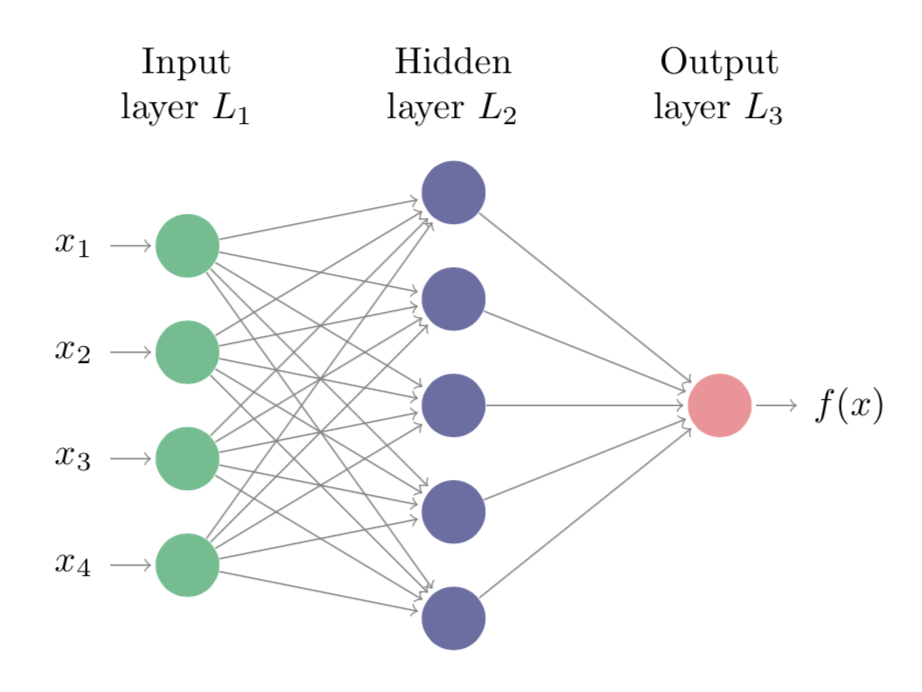
\includegraphics[width=0.6\textwidth]{images/perceptron.png}
\caption{Neural network diagram with a single hidden layer. The hidden layer derives transformations of the inputs—nonlinear transformations of linear combinations—which are then used to model the output.}
\label{fig:perceptron}
\end{figure}

\subsubsection*{Multi Layer Perceptrons}

A feed-forward neural network is a collection of neurons arranged in a sequence of multiple layers, where each neuron receive as input from the previous layer and perform a simple calculation (e.g., compute a weighted sum of the input followed by a nonlinear activation function) \cite{efron2016computer}. The neurons of the network collectively perform a nonlinear mapping from the input data to the output data. This mapping feature is learned from the data by adjusting and adapting the weights of each neuron using a technique called backpropagation \cite{efron2016computer}.

Feed Forward Neural Network Fig.~\ref{fig:multi-layer}.
\begin{figure}[htbp]
\centering
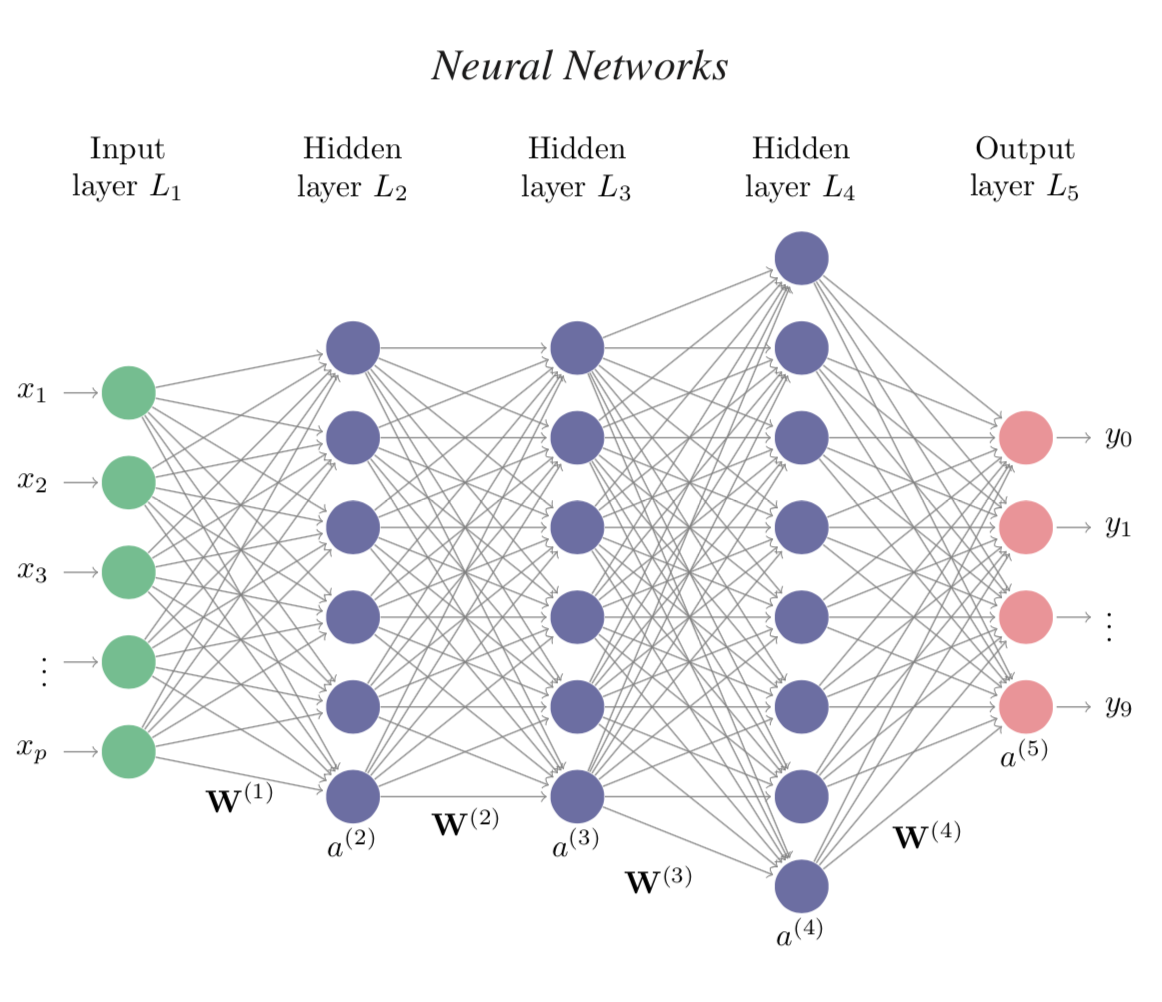
\includegraphics[width=0.8\textwidth]{images/NN.png}
\caption{Neural network diagram with three hidden layers and multiple outputs, suitable for the MNIST handwritten-digit problem. The input layer has p D 784 units. Such a network with hidden layer sizes .1024; 1024; 2048/, and particular choices of tuning parameters, achieves the state-of-the art error rate of 0:93.}
\label{fig:multi-layer}
\end{figure}

% TODO: ANN equations, weight calculation, activation units %

\subsection{Convolutional Neural Networks}
A convolutional neural network (CNN) is an image classification network in which the network preserves the hierarchical structure by learning internal feature representations and generalizing the features in tasks like object recognition and other computer vision problems. It is not restricted to images but also applicable for audio, speech and language processing problems \cite{Manaswi2018}.

An example of convolutional neural network Fig.~\ref{fig:CNN-1}.
\begin{figure}[htbp]
\centering
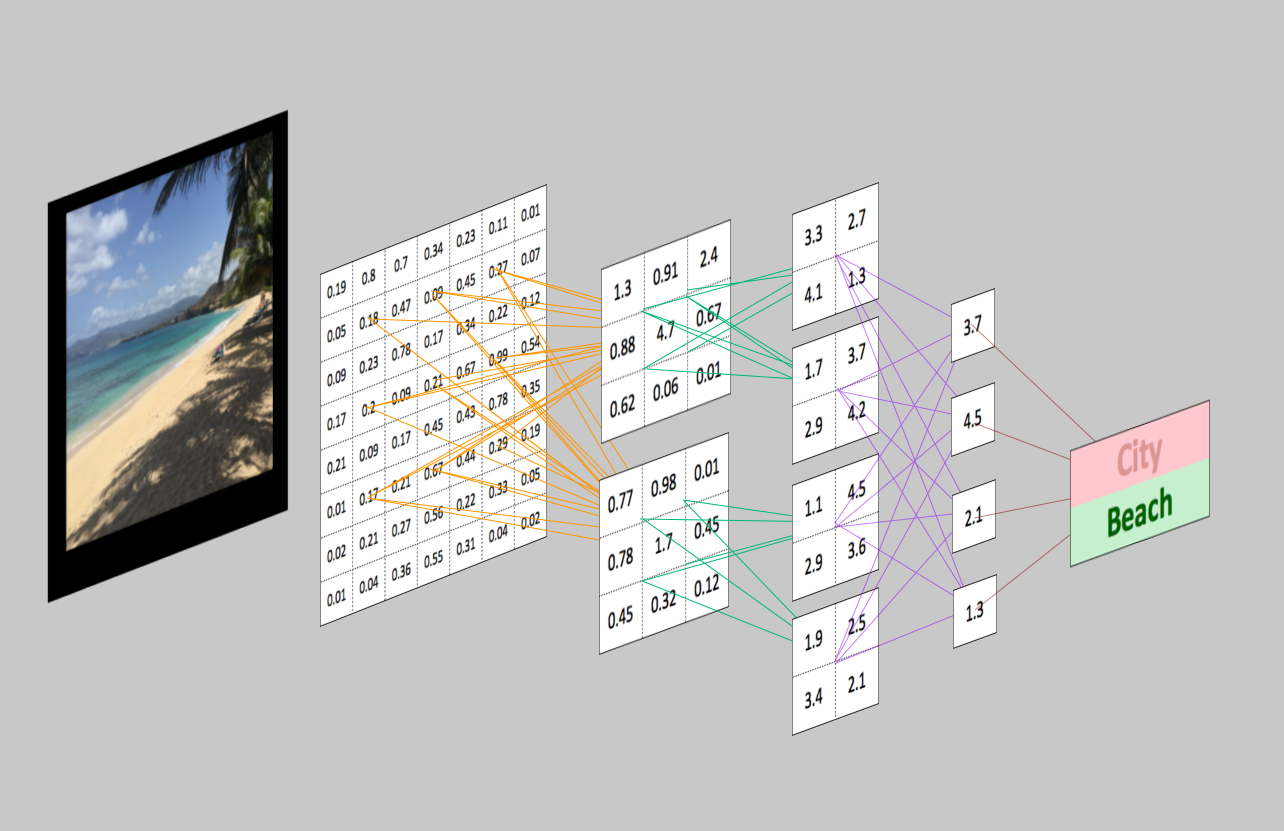
\includegraphics[width=0.7\textwidth]{images/CNN.png}
\caption{Convolutional Neural Network and computer vision}
\label{fig:CNN-1}
\end{figure}

CNN is a feed-forward deep neural network architecture comprised of a convolutional layer, each followed by a pooling layer, activation function,  batch normalization and fully connected layers. As an image passes through the network, it gets smaller and smaller due to max pooling operation. The final layer outputs the probabilities of class prediction.

Fig.~\ref{fig:CNN-1}.
\begin{figure}[htbp]
\centering
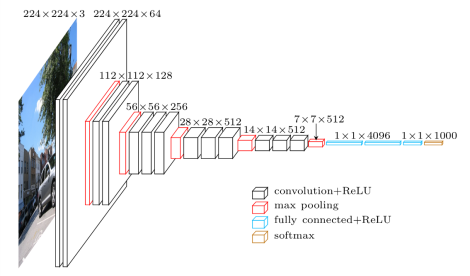
\includegraphics[width=0.7\textwidth]{images/cnn-architecture.png}
\caption{CNN Architecture}
\label{fig:CNN-1}
\end{figure}


The effectiveness of CNN in image recognition is one of the main reasons why the world recognizes the power of deep learning. As Figure 4-7 illustrates, CNN is good at building a position and rotation invariant features from raw image data. It has lead to significant advances in machine vision, which has critical applications for self-driving cars, robotics, drones, and treatments for the visually impaired.

\section{The Advent of Black Box Models}

Deep learning models are hard to interpret than most existing machine learning models \cite{Kahng2018} because of its large number of layers, myriads of parameters, multiple types of non-linear activation functions, optimization algorithms and randomized gradient descent training process; the deep neural network is often considered as “black box \cite{dlvwz}.”

Due to their internal complexities and non-linear structure \cite{Samek}, the underlying decision-making processes for why the models are achieving such performance are the challenge and sometimes mystifying to interpret. Therefore, in practice, users often use them as a black box and cannot explain how learning from input data was done nor how performance can be consistently ensured. It could also be detrimental when the model does not perform satisfactorily; users would not understand the causes or know how to fix the problem. Generally, the information stored in a neural network is a set of numerical weights and connections that provide no direct evidence as for how to the task is executed or what is the association between inputs and outputs.

\begin{figure}[htbp]
\centering
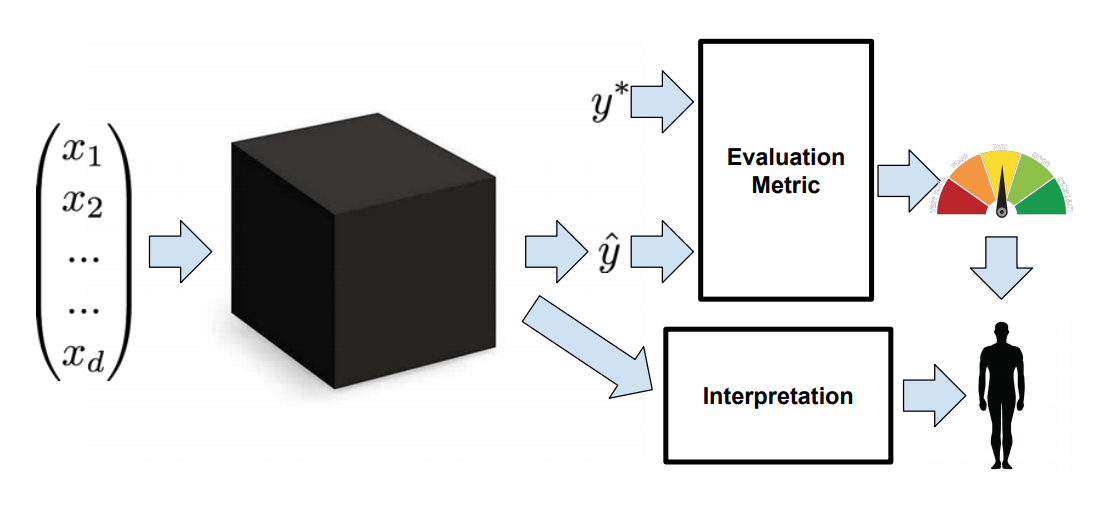
\includegraphics[width=0.90\textwidth]{images/Black-box.png}
\caption{Black box example of neural network system}
\label{fig:blackbox}
\end{figure}

The opaque nature of these models also limits their usage and acceptance in high-end science and engineering applications since it is demanded to use methods and techniques based on functions that can be understood and validated. 

Another reason that complicates the use of the neural network is that there are no well-defined criteria for choosing a neural network structure and corresponding parameter selection \cite{dlvwz}. It mostly depends on the trial and error process. The appropriate selection of parameters can vary widely even when performing very similar tasks due to various reasons. These parameters, which include network structure, depth and width of hidden layers, error bound, learning rate, training algorithm, hidden layer size, and the data vector used are often selected in a trial-and-error process. Therefore, when designing neural networks, it is tough for beginners to select the right parameters and find correct general rules. While, even for deep learning experts, it largely remains a trial-and-error process. 

The problem stems from the fact that we cannot merely inspect the deep neural network to see how it works or how it performs parallel computations \cite{darksecretaimittr}. A network’s learning and reasoning are embedded in the behavior of thousands of simulated neurons, arranged in dozens or even hundreds of intricately interconnected layers. For example, in the CNN model, neurons in the first layer receive an input image (as RGB value), which performs computation and outputs a new signal. These signals are fed into the successive layer and so on until the final layer output is generated \cite{darksecretaimittr}. Additionally, there is a process known as backpropagation that adjusts the calculation of neurons to optimize the output.

\section{Societal Implications}

As society is built upon a fabric of expected behavior and mutual trust, it is imperative we design AI systems that respect and fit with the social norms and ensure that their decision making is consistent with the ethical judgment. 

With the growing influence of artificial intelligence in our lives and their impact on the public domain, there is a critical need to understand better their decisions and realize how these models operate.  In a societal context, the reasons for a decision matters a lot. For example, death caused intentionally (murder) vs. death caused unintentionally (manslaughter) are distinct crimes at the court of law. Similarly, a hiring decision made is based (directly or indirectly) on specific protected characteristics such as race, the socio-economic class has a bearing on its legality. However, currently, predictive models are not capable of reasoning this or provide any explanation \cite{molnar}.

In this section, we examine the social implications of the black box neural network model, including how the relative opacity is potentially endangering the social equality and its wide-ranging impact in various social domains. We focus our discussion on the societal implication through seven critical themes:

\begin{enumerate}
\item \textbf{Trust}
\item  \textbf{Transparency}
\item \textbf{Fairness and Inclusion}
\item \textbf{Causality}
\item \textbf{Safety}
\item \textbf{Privacy}
\item \textbf{Ethics \& Accountability}
\end{enumerate}

We selected these themes because they are overarching concerns in the public domain. We discuss the harmful effect in each of these areas and identify emerging challenges in the present and future. In our discussion about these themes, we also ask the underlying questions such as: what are the current social and economic challenges faced by the rapid integration of AI, and how we can build a deeper understanding of AI in the present time that will help us create a fair and equitable future? \cite{Solon2017}

The wide-ranging impact in these selected themes makes it essential to look at how these automated decision-making systems are being applied now in regulated industries, whom they are benefiting, whom they are undermining, and how they are structuring the socio-economic aspect of society and individuals \cite{ainow2016report}.

\subsection{Trust}

For humans, It is easier to trust a system that explains its decisions compared to a black box. Deep learning to be confidently rolled out by industries and governments, users want greater transparency through explanations and justification of its decisions \cite{molnar}. It is an essential condition, not only for risk management but also to establish greater trust from the general public as well as regulators and supervisors in financial services. 

\subsection{Transparency}

Transparency is the opposite of opacity or the notion of black box”. Transparency is considered here at the level of the entire model at the level of individual components such as parameters (decomposability), and the level of the training algorithm (algorithmic transparency). 

\subsection{Fairness and Inclusion}

It is important to ensure that predictions made by the models are unbiased and do not implicitly or explicitly replicate human bias or discriminate against protected groups \cite{ainow2016report}. An interpretable model can explain why it decided to deny a loan for a particular person, and it becomes transparent and more accessible for a human to judge whether the decision made by the model is based on a learned demographic or not.

\subsection{Causality}
The model should ensure that it considers only causal relationships.  The system can only be compromised if the inputs are proxies for a causal feature, but do not cause the outcome. Hence proxy features should be avoided as they make models vulnerable. (\cite{molnar})

\subsection{Ethics}

Ethical questions surrounding AI systems are wide-ranging, spanning creation, uses and outcomes. There are important questions about which set of values and interests are reflected in AI, as well as how machines can recognize values and ethical paradigms. AI ethics concerns broader social concerns about the effects of AI systems and the choices made by the people who developed it.

\subsection{Privacy}
Assuring that sensitive information in the data is protected and uncompromised is important for privacy and security \cite{molnar}. AI challenges current understandings of privacy and strains the laws and regulations we have in place to protect personal information. Established approaches to privacy have become less and less effective because they are focused on previous metaphors of computing, ones where adversaries were primarily human. AI systems’ intelligence, as such, depends on ingesting as much training data as possible. This primary objective is adverse to the goals of privacy. AI thus poses significant challenges to traditional efforts to minimize data collection and to reform government and industry surveillance practices. 

\subsection{Safety}
Interpretability is especially critical if we want to consider autonomous vehicle safety before deploying the system, e.g., if specific errors are unacceptable even during training like specific edge case testing for self-driving cars. This aspect extends beyond autonomous vehicles to general AI systems, weighing in what kind of understanding is most helpful for safety?

\subsection{Accountability}
Terminology is now further complicated by concerns over the accountability (Diakopoulos 2016) and fairness (O’Neil 2016) of modern AI systems which, while overlapping the issue of end-user trust, extend into ethical and legal domains. It is important to ensure that small changes in the input do not lead to large changes in the prediction.

\section{Explainable and Interpretable System}

Interpretability is defined as the point to which a human can understand the causes of a decision. Another definition is that Interpretability is the degree to which a human can consistently predict the model’s result \cite{molnar}. The higher the interpretability of a machine learning model, the easier it is for someone to comprehend why certain decisions or predictions have been made. A model is better interpretable than another model if its decisions are more accessible for a human to comprehend than decisions from the other model \cite{molnar}.
    
Interpretability is the process of generating humanly understandable explanations of why a deep learning model makes a particular decision. Since the learning system hides the entire decision process behind the complicated inner-workings of deep learning models, it becomes difficult to obtain interpretations and explanations for their decisions.

As deep learning become an indispensable tool for a wide range of applications, it is essential to be able to verify for a certain task that the accuracy results from the proper framing of a problem statement, and there is no exploitation of artifacts in the data. Techniques for interpreting and understanding what the model has learned have therefore become a key ingredient of a robust validation procedure \citep{taylor2006methods} \citep{hansen2011visual} \citep{bach2015pixel}. Interpretability is critical in applications such as medical diagnosis or self-driving cars, where the dependency of the model on the correct features should be guaranteed \citep{Caruana:2015:IMH:2783258.2788613} \citep{bojarski2017explaining}.

\subsection{Why Interpretability Matters}

While artificial intelligence (AI) has existed for over sixty years, but the real-world application has increased only in the last decade due to factors discussed in the above section: the recent surge in data and the rise in computing power together with better algorithms.

With the growing success of deep learning and neural networks, there is a corresponding need to be able to explain their decisions, which includes detecting model bias, establishing trust and building confidence about how it performs in a real-world situation.

Without a clear understanding of how and why a model works in a certain way, the development of these models relies on a time consuming trial-and-error process. Consequently, both researchers and practitioners are facing challenges with complex models that demand more transparency and explainable systems to better understanding and analysis of these models. Whether it's an financial decision, a medical decision or maybe a military decision, one cannot rely on a black box method. It's time to act on making these decisions more transparent and understandable before the technology becomes even more pervasive.

This issue of black box neural networks has been a primary concern and a significant focus of discourse in the last few years among researchers and practitioners \cite{Samek}. As deep learning spreads across domains, it is of paramount importance that we equip users of deep learning with tools for understanding when a model works correctly, when it fails, and ultimately how to improve its performance.

\iffalse
The 2017 report from the AI committee of the British parliament states that the development of the intelligence AI systems is a fundamental necessity if an AI system is to become an integral and trusted tool in the society. Whether it takes the shape of explainability, technological transparency or both depend on the context and stakes involved in its application. However, in most cases, the report ascertains, explainability to be a useful approach for the citizens and the consumers. Further, the report suggests that it is not acceptable to implement an artificial intelligence system that could have a substantial impact on an individual's life unless it can provide a full, comprehensive and satisfactory explanation for the decisions it makes. It means delaying their deployment for such use cases until a credible alternative solution is found.
\fi

\subsection{Explainable Artificial Intelligence}
XAI concept explains individual decisions, enables understanding of overall strengths and weaknesses, and conveys an understanding of how the system will behave in the future and how to correct the system’s mistakes.

\begin{figure}[htbp]
\centering
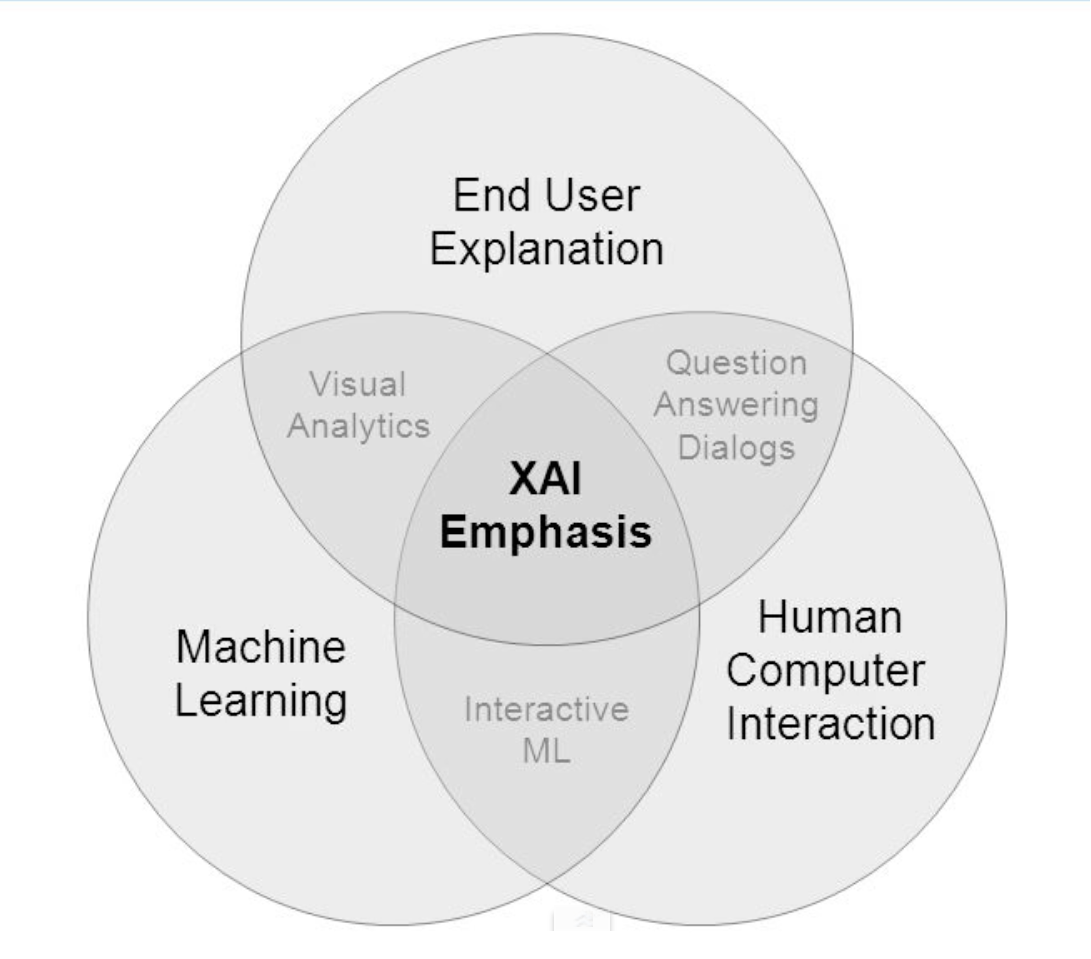
\includegraphics[width=0.65\textwidth]{images/XAI Research-1-crop.png}
\caption{Emphasis and Scope of XAI Research}
\label{fig:xai-1}
\end{figure}

Explainable Artificial Intelligence (XAI) System:  There has been a wave of interest in explainable artificial intelligence (XAI) in recent years driven by DARPA’s initiative to fund XAI projects. Historically, there has been occasional interest in explanations of intelligent systems and automated decision making systems over the past decades with expert systems, designed to solve complex problems by reasoning through prior knowledge in the 1970s [165, 172], Bayesian networks and artificial neural networks [6] in the 1980s, and then the recommender systems in the 2000s [33, 81]. The recent successes and advancement of AI and machine learning for many large-scale applications and the use of increasingly complex and non-transparent algorithms, mainly deep learning, calls for another rise of interest for the need to better understand these systems.

\section{Deep Learning Visualization Research}

With the growing complexity of AI models, the critical need for understanding their inner-workings has increased. Visualization is potentially a powerful technique to fill such a critical need. It can help bring more insight into the often obfuscated complex AI systems.
% TODO: NEED VISUALS

More than ever, data visualization has become critical to the field of AI. It can potentially help three broad groups of practitioners and users of AI who stand to benefit from deep learning visualization and visual analytics: model developers, model users, and non-experts \ref{Choo2018}.

Deep learning visualization research is an interdisciplinary area involving both deep learning and visual analytics techniques \cite{Choo2018}. It is distributed across multiple related fields within and outside the deep learning and AI community. In academia, the primary venue for deep learning visualization research consists of two main groups (1) Information Visualization and Visual Analytics community; and (2) artificial intelligence and deep learning communities. 

In addition to that, since this area is relatively new and emerging \cite{Choo2018}, it has seen more attention at multiple conferences and workshops, such as Neural Information Processing Systems (NeurIPS), IEEE Transactions on Visualization, IEEE Information Visualization and Computer Graphics and ICML Workshop on Human Interpretability in ML as just to name a few examples.

\subsection{Information Visualization Elements}

Information visualization is the study and usage of visual representation of abstract data to reinforce human cognition. It can help with the discovery of unstructured actionable insight, exploring and understanding the patterns in the data to communicate essential aspects of your data set in a concise, easy-to-understand fashion.

Data analysis is an indispensable part of the machine learning project pipeline, in both academia and research; and industry projects. The AI development pipeline often begins with data exploration phase, also known as exploratory data analysis to help with data analysis and evaluate approaches for the problem at hand. It has primarily been done using fundamental data analysis approach in visualization such as histograms, plots, charts, graphs and other types.

\subsection{Visual Analytics System}
    
Visual Analytics combines information visualization and scientific visualization and focuses on the analytical reasoning enabled with interactive visual interfaces. It’s an amalgamation of computer science, information visualization, cognitive and perceptual sciences, interactive design and social science.

Visual Analytics system have been developed to inspect artificial neural networks since visual feedback is considered highly valuable by both the practitioners and researchers


\subsection{Visualization and Interpretability}

Visualization is a powerful tool to meet this critical need. It can be used to demystify Deep Learning and explain how AI techniques work. Interactive Visualization would help enhance the interpretability and explainability of the deep learning models. Interactive visualization or Visual Analytics, as a whole is emerging as a promising research field. It has the potential to provide an in-depth understanding of deep learning models work and help make their inner workings transparent.


    \chapter{METHODOLOGIES}

\graphicspath{ {./methodologies/} }
%%%%%%%% This line gets rid of page number on first page of text
\thispagestyle{empty}

%%%%%%%%%%%%%

\section{Method Selection}

The methodologies section covers methods chosen to investigate the research problem. We begin this section by restating our research problem and underlying assumptions underpinning our study: interpreting and understanding deep neural networks using interactive visualization, to inspire human curiosity and learning among the non-technical audience, as well as broaden people's access to interactive tools for deep learning.

\subsection{Scientific Methods}

The primary method selected for the research process is the scientific method. We selected this method as it involves careful observation and empirical study.

As deep learning is essentially a method for machines to learn from data and classifying patterns that is loosely modeled on the way a biological brain learns to solve problems. The scientific method is aptly suited for this type of research as it involves careful observation and empirical study of the topic in question, which includes rigorous skepticism about what is observed and iterative testing and experimentation to validate or invalidate it.

The underlying principles of the scientific method \cite{gauch_jr_2012} are essential for evaluating the hypothesis, enhancing perspective, increasing productivity, and inspiring innovation. These principles include logic, probability, parsimony and hypothesis testing, as well as science's presuppositions, limitations, principles and bold claims of rationality and truth. Beyond such methodology, some practical issues are shared broadly across the sciences, such as implementing effective science education and relating the scientific enterprise to the humanities.

The scientific method consists of two stages \cite{2016397}: the first consists of formulating hypotheses, and the second consists of testing them. What differentiates this from other forms of methods is the second stage: subjecting hypotheses to empirical testing by ascertaining whether or not predictions derived from hypotheses are borne out in relevant observations and experiments. Hypotheses and assumptions are the initial stages of scientific inquiry because they incentivize seeking truth and a hint as to where to find it. \cite{AYALA2016xi}

Additionally, we also employed other research methods to bolster our research processes, such as action as research, agile development and system design. The selection of a research methodology was dependent on the research question itself and how best it can be addressed: interpreting deep neural networks.

\subsection{Action Research}
Action Research is a research methodology driven by practical problems, emphasis participatory research, and develops practically useful solutions to a real-world problem iteratively. It offers a systematic, collaborative approach to conducting research that satisfies both the need for scientific rigor and promotion of sustainable social change and has been taken up by a variety of researchers in both academic and industrial settings. \cite{Hayes:2011:RAR:1993060.1993065}

Action Research emphasizes the knowledge produced in the context of the application (Lewin, 1946; Susman \& Evered, 1978). It’s a distinct candidate research method when the objective is to explore theory concerning practice.

\section{Research Hypothesis}

While deep neural networks learn efficient and powerful representations, they are often considered a ‘black-box.’ In most cases, they learn representation that is difficult to extract and present in a human-readable form. While it can be true for certain types of deep learning models, it is not entirely true for some of the popular networks like a convolutional neural network, recurrent neural network, semi-supervised and unsupervised method.

\section{Hypothesis Testing}

<REWRITE> Building upon our research question stated in the above section; we formulated our hypothesis as follows -  Develop a prototype that serves a set of utilities or toolkit for interpreting a visual classifier by providing visual evidence for their decision using interactive visualization.

\section{Prototype Objective}

<REWRITE> The prototype is intended and designed for people with a non-technical background to understand the fundamental concepts of the neural network, in our case, a visual classifier. Our objective can be summarized mainly as (1) Explanation of neural networks for people with a non-computer science background (2) Inspire curiosity and learning among non-technical audiences  (3) Broadens people's access to interactive tools for deep learning.

\section{Technical Design}
The following segment provides an overview of the technical design and resources required for the successful development of the prototype. It provides a high-level overview of the components in scope, functionality, dataset and environmental setup.

\subsection{Model Selection}

<REWRITE> As model selection is the centerpiece of the data science workflow, we evaluated a set of candidate pre-trained models by running a series of the experiment. It mainly helped us assess if the data collected is well suited to the problem of model selection. We also considered the hyperparameter setting and other configuration details required to fit the model. We also tested the compatibility of the model with the available public dataset. Based on our evaluation we selected VGG-16 as the primary model for the prototype development. This model is trained on the imagenet database.

VGG-16 is based on convolutional neural network model proposed by the Visual Geometry Group from the University of Oxford in the paper “Very Deep Convolutional Networks for Large-Scale Image Recognition”.  The model achieves 92.7\% top-5 test accuracy in ImageNet, which is a dataset of over 14 million images belonging to 1000 classes. It was one of the famous model submitted to ILSVRC-2014 competiton. This is used as the backbone network in our project.

A schematic view of Visual Geometry Group 16 Model.~\ref{fig:CNN-1}.
\begin{figure}[htbp]
\centering
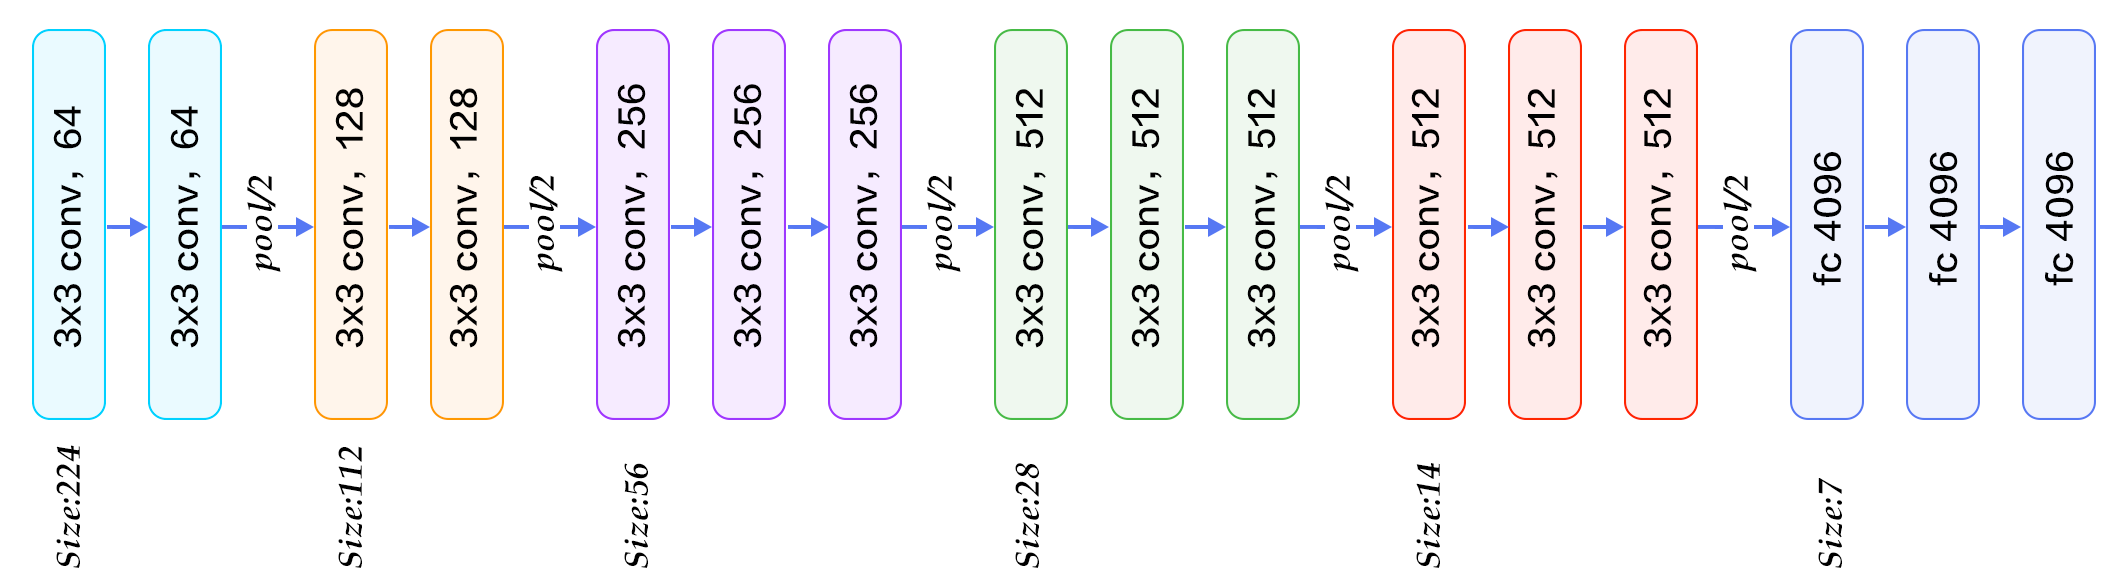
\includegraphics[width=1\textwidth]{images/cnn-vgg16-1.png}
\caption{VGG16 hidden layers}
\label{fig:CNN-1}
\end{figure}

\subsection{Dataset}

ImageNet database consist of over 15 million labeled high-resolution images that belong to roughly 22,000 categories. These images were downloaded from Google image search and labeled by humans using Amazon's Mechanical Turk crowd-sourcing tool in 2012. It took about two and half years to label all the images. The labeled dataset was first introduced in a competition called the ImageNet Large-Scale Visual Recognition Challenge (ILSVRC). The competition used a subset of ImageNet with around 1000 images in each of 1000 categories. In total, there are 1.2 million training images, 50,000 validation images, and 150,000 testing images. To maintain consistency of resolution, images have been down-sampled to a fixed resolution of 256x256 dimensions.
    
\subsection{Framework Selection}

<REWRITE> To develop client-side deep learning application, we surveyed several open source machine learning framework for the web such as TensorFlow, Keras, PyTorch, Caffe and WebDNN. Based on our assessment and feedback from the developer community, we found TensorFlow.js as a right choice for training and inference of deep learning models on the browser. Additionally, Tensorflow.js is feature-rich and takes advantage of GPU-accelerated training processes. 

<REWRITE> We use TensorFlow and TensorFlow.js library, released by Google in Mar. 2018 is an in-browser open source machine learning framework that supports defining, training and running deep learning models in the browser using JavaScript (JS). It is the successor of the deeplearn.js which is now called TensorFlow.js Core. 

<REWRITE> While several other open source JS platforms for machine learning have appeared in recent past, to our knowledge, TensorFlow.js is commonly used and have enabled developers to create interactive and explorable explanations for deep learning models on the web.

<REWRITE> TensorFlow.js leverages GPU processing power to accelerate deep learning tasks on browsers via WebGL. WebGL is a back-end compute on GPU by WebGL API, which is a JavaScript API for rendering interactive 2D and 3D graphics within any modern compatible browsers. TensorFlow.js provides a low-level core API to perform linear algebra operations and automatic differentiation, and high-level Layers APIs for building and training models. The layers used in Tensorflow.js support the Tensorflow and Keras layers in the native platform. Supported features also include conversion of models built in the native platform, importing pre-trained models for inference and retraining imported models.

\subsection{Visual Exploration Tool}

DeepViz is a visual exploration tool targeted towards the non-technical audience to explore the inference (or predictions) made by a visual classifier, an image recognition deep learning model.

Deep learning in the browser is at the experimental stage and recently a bunch of JavaScript-based deep learning framework has been introduced, making it possible to perform several deep learning tasks directly on the browser. Some of the supported features include model training, importing pre-trained models, transfer learning and inferences.

However, there is a debate on the feasibility and effectiveness of the web-based deep learning applications. One one hand, those who object think browsers are not primed for running deep learning tasks and its merely impractical due to the poor performance of client-side scripting and limitations imposed by the browsers. 

On the other hand, advocates think that the browser is an ideal platform for realizing client-side machine learning that allows highly rich interaction and improves personalization for end users. The benefits include but not limited to faster user interaction, preserving data privacy, lower back-end payload, reduced data transfer and performance latency of HTTP client-server communication.

\section{Computational Environment}

\subsection{Client-side Neural Network Overview}
Developing AI applications using modern deep learning framework is a non-trivial task. Normally these frameworks and libraries are leveraged by native applications that run on a native platform environment such as Linux, Windows, MacOS/iOS and Android. Thus most production-level libraries are developed for and written in Python, Java and C++. 

Developing AI application that is cross-platform and portable on multiple devices is not easy. The development of a native application is an intricate and time-consuming process. It is particularly complicated for mobile applications as the app vendors usually need to develop and maintain both iOS and Android version, in addition to the desktop application.

Compared to the native application, client-side applications can make the portability issue simpler for the cross-platform. The sample implementation of deep learning powered web application can be deployed on multiple platforms regardless of operating systems, hardware or device types.

\subsection{Supported Browser Features}
We analyzed the supported browser features for machine learning tasks and taken into consideration the factors that may affect the efficiency when building and deploying deep learning application on the web. One of them is the debugging capability to support model and data inspection when running deep learning tasks.

Further, in-browser deep learning allows users to use their local data and then train the model directly in the browser, which means there is no back-end end or server is necessary. 

\section{Experimental Setup}

We set up the development environment for building the client side application using JavaScript ES6, Node.js and Tensorflow.js. We download the required modules and dependencies, including tensorflow.js, D3, transpiler to convert code written in JavaScript ES6 into plain old ES5 JavaScript that can run in any browsers. We use Webpack and Bitbucket for bundling and deployment.

\iffalse
\section{Infrastructure and Tooling}
\subsection{GPU Acceleration}
\subsection{Hardware}
\subsection{Software}
\subsection{Build and Tooling}
\subsection{Cloud computing services}

\subsection{Base Architecture}
\subsection{Model Conversion}
\subsection{Dataset}
\subsection{Data Pre-processing}
\subsection{Parameter Settings}
\subsection{Application Prototype}
\subsection{Real-time processing}
\fi
    \chapter{RESULTS}

\graphicspath{ {./results/} }
%%%%%%%% This line gets rid of page number on first page of text
\thispagestyle{empty}

%%%%%%%%%%%%%

The result section details essential findings from our research study and prototype testing, including multiple iterations and user testing to analyze different variations.

\section{Visual Analysis}

The critical finding from the research highlights that the representations learned by the VGG16 image recognition model are highly amenable to visualization, in large part because they are representations of visual concepts. 

Although a wide variety of techniques are under development in the research and visual analytics community, we covered three of the most accessible and useful ones:

\begin{enumerate}
\item Visualizing heatmaps of class activation
\item Visualizing filter patterns
%\item Visualizing intermediate activations
\end{enumerate}

For all three methods, we use the VGG16 model, a convolutional neural network based model trained on the imagenet database that we introduced in the previous section.

\section*{Visualizing heatmaps of class activation}

This step helps to understand precisely which part of an image identified to belong to a specific class or category (class names known to VGG16), and thus allows localizing objects in images.

We feed the following image of a group of bee-eater sitting on a tree branch as an input image.

Input image ~\ref{fig:myFig}.
\begin{figure}[htbp]
\centering
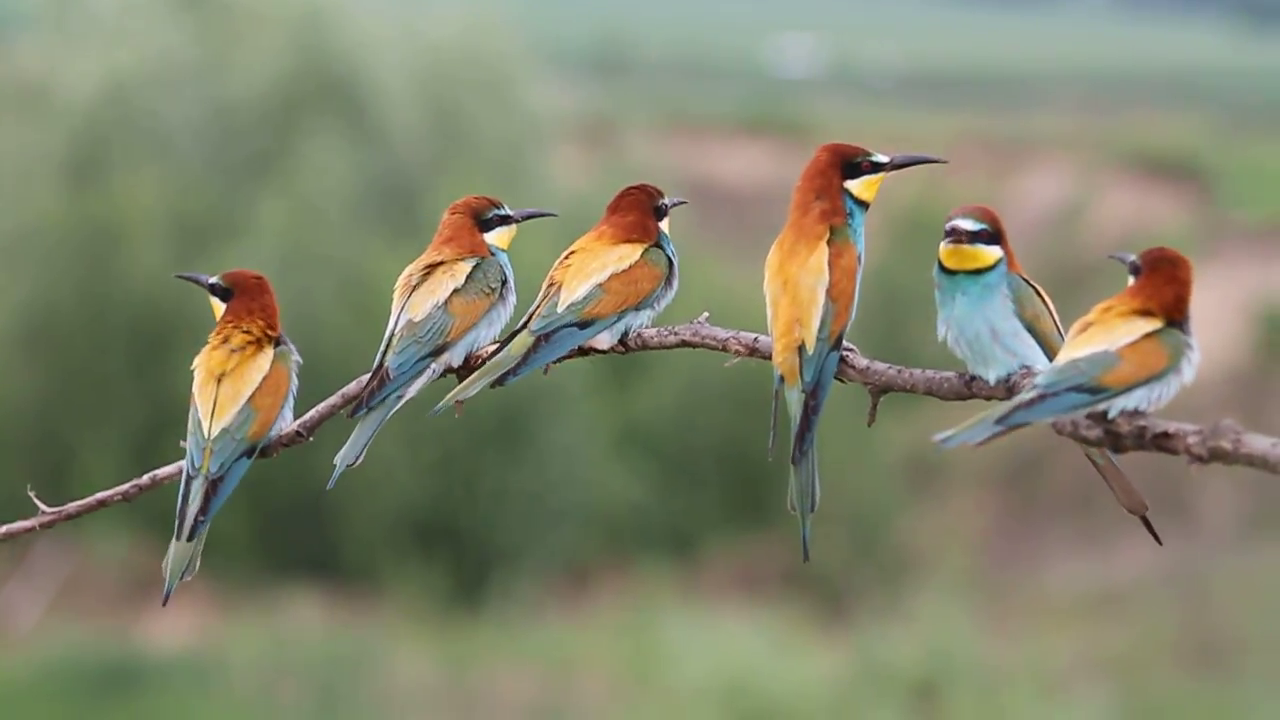
\includegraphics[width=0.80\textwidth]{images/colorful-group-of-birds-get-together_vkmuak6_e__F0000.png}
\caption{An image of colorful group of birds uploaded by the user}
\label{fig:myFig}
\end{figure}

>>> [IMAGE] Rooster Image (EXPLAINABLE ARTIFICIAL INTELLIGENCE: UNDERSTANDING, VISUALIZING AND INTERPRETING DEEP LEARNING MODELS)

Class activation heatmap~\ref{fig:heatmap-1}.
\begin{figure}[htbp]
\centering
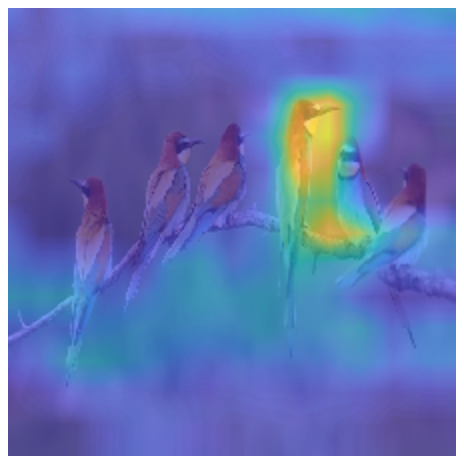
\includegraphics[width=0.60\textwidth]{images/heatmap-class-activations.png}
\caption{Sensitivity Analysis}
\label{fig:heatmap-1}
\end{figure}

\section*{Visualizing filters}

This step that visualizes set of patterns, which is useful to understand precisely what visual patterns or concepts each filter in a layer is receptive to.

\section*{Visualizing intermediate activations}

This step helped to understand when fed with an input image, how successful layers of the network transformed the input image. It also helped get an idea of the meaning of the individual network filters.

\iffalse
Figure 3~\ref{fig:layer-activation}.
\begin{figure}[htbp]
\centering
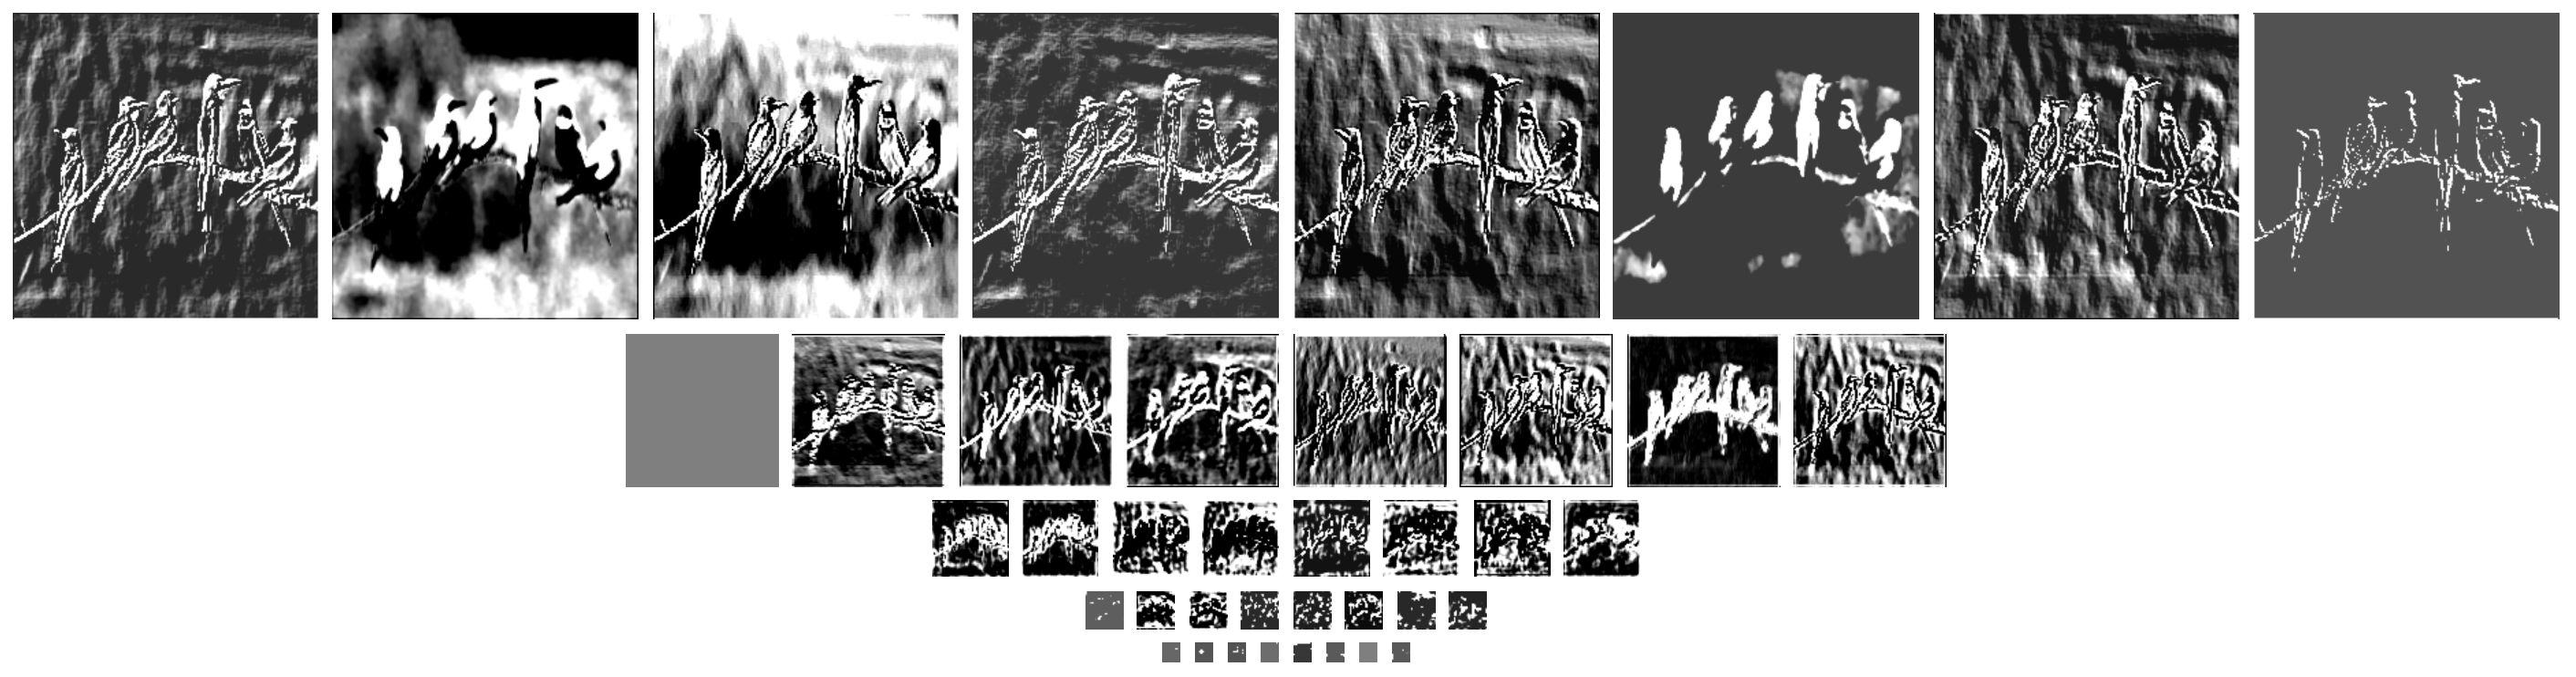
\includegraphics[width=1\textwidth]{images/layer-activations.png}
\caption{Intermediate outputs}
\label{fig:layer-activation}
\end{figure}
\fi

Our visualization technique helped to answer two important questions:

\begin{itemize}
\item  Why did the network think this image contained a bee-eater?
\item Where is the bee-eater located in the picture?
\end{itemize}

In particular, what is most exciting to note is that the head region of the fourth bird, which is the largest of all six birds are strongly activated: this is probably how the network can tell the difference between bee-eater and any other bird.

% TODO: USER STUDIES%

\ifalse
RESULTS___
WE USE localization approaches like CAM APPROACH ONLY + ....

Visualizing intermediate activations¶

Visualizing intermediate activations consists in displaying the feature maps that are output by various convolution and pooling layers in a network, given a certain input (the output of a layer is often called its "activation", the output of the activation function). This gives a view into how an input is decomposed unto the different filters learned by the network. These feature maps we want to visualize have 3 dimensions: width, height, and depth (channels). Each channel encodes relatively independent features, so the proper way to visualize these feature maps is by independently plotting the contents of every channel, as a 2D image. Let's start by loading the model that we saved in section 5.2:

Visualizing convnet filters
inspect the filters learned by convnets is to display the visual pattern that each filter is meant to respond to. This can be done with gradient ascent in input space: applying gradient descent to the value of the input image of a convnet so as to maximize the response of a specific filter, starting from a blank input image. The resulting input image would be one that the chosen filter is maximally responsive to.

Visualizing heatmaps of class activation¶
We will introduce one more visualization technique, one that is useful for understanding which parts of a given image led a convnet to its final classification decision. This is helpful for "debugging" the decision process of a convnet, in particular in case of a classification mistake. It also allows you to locate specific objects in an image.
This general category of techniques is called "Class Activation Map" (CAM) visualization, and consists in producing heatmaps of "class activation" over input images. A "class activation" heatmap is a 2D grid of scores associated with an specific output class, computed for every location in any input image, indicating how important each location is with respect to the class considered. For instance, given a image fed into one of our "cat vs. dog" convnet, Class Activation Map visualization allows us to generate a heatmap for the class "cat", indicating how cat-like different parts of the image are, and likewise for the class "dog", indicating how dog-like differents parts of the image are.
\fi

\iffalse
\section{Visualization Outcome}
\section{Statistical Analysis}
\section{Visual Analysis}


\section{User Testing}
\section{Performance Testing}
\fi

    %
%  This is an example of how a LaTeX thesis should be formatted.  This
%  document contains chapter 1 of the thesis.
%

\chapter{CONCLUSION}
%%%%%%%% This line gets rid of the page number on the first page of text
\thispagestyle{empty}
%%%%%%%%%%%%%

%INJECT[The first paragraph in the Discussion should summarize the Results. Most readers will read the Abstract, maybe the Introduction, and then the Discussion. Write the Discussion as if it were the first thing your readers saw.]

%INJECT[Then you need 2-3 paragraphs placing your results into a broader context. What does your work mean for the major question described in the Introduction? Also, how does your work relate to other work in the field? What specifically are the similarities and differences?]

%INJECT[Finally, and this is somewhat optional, you can write another paragraph that summarizes all your findings once more]

Research in deep learning has traditionally focused on new algorithms, mathematical models, improving quality and performance or the speed of the neural network model. I have studied and investigated a lateral research direction that touches upon the social implication of the automated decision-making systems, namely, we have contributed to furthering the understanding and transparency of the decision making implemented by a trained deep neural network. 

I proposed a visual exploration tool for interpreting a visual classifier that provides a visual explanation of the inference decision. The tool is targeted towards non-experts and helps broaden people's access to an interactive tool for deep learning. The visualization technique helps make an image recognition model more transparent by providing a visual explanation for its predictions. My prototype helped to answer two critical questions about model inference raised in our research hypothesis: (i) why did the network think this image contained a specific object (ii) where is the object located in the picture. I used the heatmap concept that allowed better intuition about what has been learned by the network.

Further, running deep learning application entirely client-side in the browser unlocked new opportunities to add rich interaction and user experience. From a user's perspective, there is no need to install any libraries or drivers. They can directly access the application in their browser. Finally, all the user data stays on the client-side local to the user device, and this helps to maintain as a privacy-preserving application.

In summary, I have presented a novel image explanation technique that justifies the class prediction of a visual classifier. This method could be a  stepping stone and serve as a foundation for a more robust model interpretability and explainable system. This work is a small contribution towards building a fair, transparent and explainable AI system


    
    % Endmatter
    % For BibTeX references: specify a .bib file and a style.
    % The style used here is for IEEE transactions formatting:
    \references{IEEEabrv,reference}{IEEEtran}
    % The style used here is for AIAA formatting:
%    \references{IEEEabrv,sample}{aiaa}
    
    %
%  Example Appendix pages.
%  Modified to use new usu-thesis-mk2 appendix facilities.
%
%  Time-stamp: "[appendix.tex] last modified by Scott Budge (scott) on 2011-08-08 (Monday, 8 August 2011) at 15:46:06 on goga"
%
%  Info: $Id$   USU
%  Revision: $Rev$
% $LastChangedDate$
% $LastChangedBy$
%
%
% For a single appendix, use \makeappendix, and place the 
% body of the appendix after it

%\makeappendix

% < single appendix body here >

% For multiple appendices, use \makeappendices, and create each appendix
% using \appendix{}
% For sub-appendices use \appendixsection{} and \appendixsubsection{}

\makeappendices
\appendix{Summary Tables}
\label{chap:appendix}


\appendixsection{VGG16 Model}
\label{sec:vgg16-layers}

A model summary and list of hidden layers in VGG16 in Table~\ref{table:vgg16-layer}.

\begin{table}[!t]
% increase table row spacing, adjust to taste
  \renewcommand{\arraystretch}{1.3}

  \caption{List of hidden layers in the VGG16 model}
  \label{table:vgg16-layer}

  \centering
  \begin{tabular}{|c|c|c|} \hline
  
     Layer (type) & Output shape & Parameters \\ 
     \hline

    
    input1 (InputLayer) & \lbrack null,224,224,3\rbrack & 0 \\
    \hline
    
    block1 conv1 (Conv2D) & [null,224,224,64] & 1792 \\
    \hline
    
    block1 conv2 (Conv2D) & [null,224,224,64] & 36928 \\
    \hline
    
    
    block1 pool (MaxPooling2D) & [null,112,112,64] & 0 \\
    \hline
    
    block2 conv1 (Conv2D) & [null,112,112,128] & 73856 \\
    \hline
    
    block2 conv2 (Conv2D) & [null,112,112,128] & 147584 \\
    \hline
    
    block2 pool (MaxPooling2D) & [null,56,56,128] & 0 \\
    \hline
    
    block3 conv1 (Conv2D) & [null,56,56,256] & 295168 \\
    \hline
    
    block3 conv2 (Conv2D) & [null,56,56,256] & 590080 \\
    \hline
    
    block3 conv3 (Conv2D) & [null,56,56,256] & 590080 \\
    \hline
    
    block3 pool (MaxPooling2D) & [null,28,28,256] & 0 \\
    \hline
    
    block4 conv1 (Conv2D) & [null,28,28,512] & 1180160 \\
    \hline
    
    block4 conv2 (Conv2D) & [null,28,28,512] & 2359808 \\
    \hline
    
    block4 conv3 (Conv2D) & [null,28,28,512] & 2359808 \\
    \hline
    
    block4 pool (MaxPooling2D) & [null,14,14,512] & 0 \\
    \hline
    
    block5 conv1 (Conv2D) & [null,14,14,512] & 2359808 \\
    \hline
    
    block5 conv2 (Conv2D) & [null,14,14,512] & 2359808 \\
    \hline
    
    block5 conv3 (Conv2D) & [null,14,14,512] & 2359808 \\
    \hline
    
    block5 pool (MaxPooling2D) & [null,7,7,512] & 0 \\
    \hline
    
    flatten (Flatten) & [null,25088] & 0 \\
    \hline
    
    fc1 (Dense) & [null,4096] & 102764544 \\
    \hline
    
    fc2 (Dense) & [null,4096] & 16781312 \\
    \hline
    
    predictions (Dense) & [null,1000] & 4097000 \\
    \hline

  \end{tabular}

\end{table}


%\textbf{Total parameters}: 138357544 \newline
%\textbf{Trainable parameters}: 138357544 \newline
%\textbf{Non-trainable parameters}: 138357544 \newline

\appendix{Appendix}

%\appendixsection*{Background}
%\label{sec:back}

%\appendixsection*{Methodologies}
%\label{sec:meat}



    %}}}
\end{document}
